\section{Vehicle Design and Development}
  Finalisation of the chosen concepts for the development of the rover meant that the project could progress to the detailed design stages. It was discussed in Section~\ref{subsubsec:central-control-system} that the mechanical design of the vehicle would be driving of the project, specifically the software aspects, and thus the report will deal with the mechanical and electronic detailed design first.
  
  \subsection{Mechanical Design}
    The mechanical design was initiated by planning the basic layout of mechanical subsystems and components and from that point developing each system further. In this section, the choice of scale (and hence dimensions) is followed by the overall plan of mechanical layout. Subsystems that were peripheral to the body structure are then covered, which include the suspension, differential and mast subsystems. Finally, the design of the body structure is described as well as detail surrounding the model as a whole.
    
    \subsubsection{Scale and Dimensions}
      Replication of \textit{Curiosity} on an aesthetic level was a project aim to increase the viewers' and users' sense of familiarity with the model, a way of promoting the engaging experience. The replication process identified that proportion was an effective and achievable starting point and it was decided that as many of the parts as possible be based off the dimensions of the corresponding part on \textit{Curiosity}, brought down to scale by a predetermined factor. Scale was constrained primarily by the cost and manufacturing time of parts that were required to be 3D printed; the larger the model, the greater the amount of material required and the longer it would take to print it. The print bed size was also a constraint in this regard. More details pertaining to the use of 3D printing facilities can be found in Section~\ref{subsubsec:additive-manufacture}.
      
      \begin{figure}[h]
        \centering
        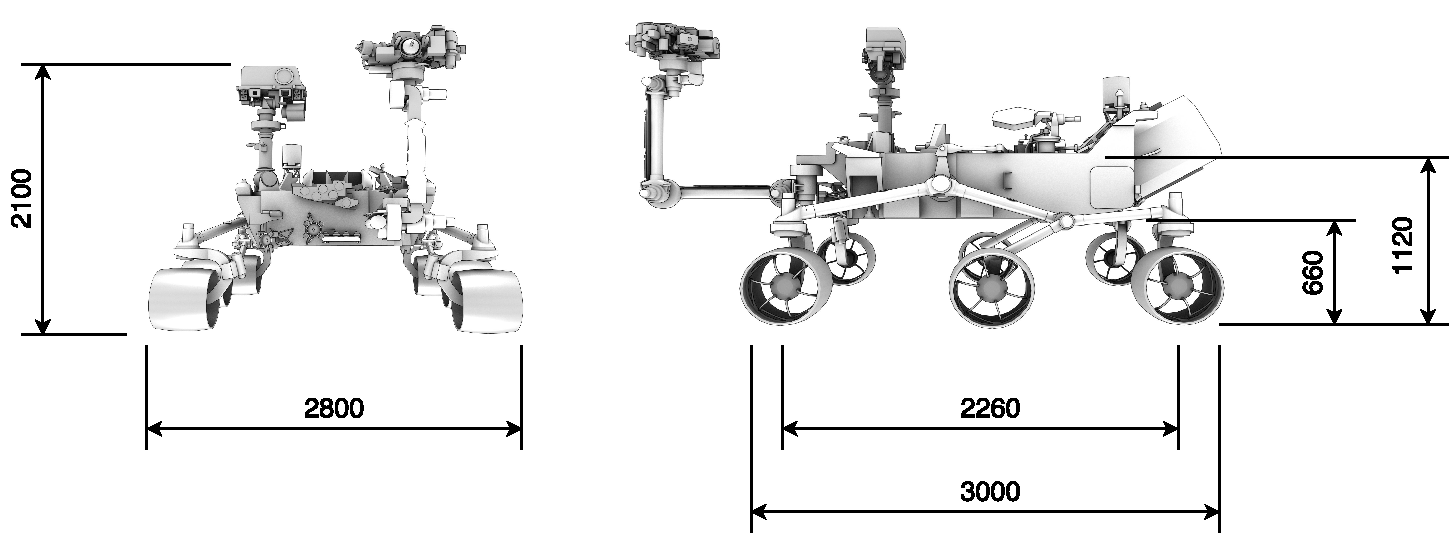
\includegraphics[width=0.9\linewidth]{figures/mechDesign-curiosityDimensions}
        \caption[Diagram indicating the external dimensions of \textit{Curiosity} in millimetres]{Diagram indicating the external dimensions of \textit{Curiosity} in millimetres \cite{nasa3D}}
        \label{fig:mechdesign-curiosityDimensions}
      \end{figure}
      
      The dimensions shown in Figure~\ref{fig:mechdesign-curiosityDimensions} were retrieved from \cite{nasajulypresskit} and \cite{roverThermal_2016} as guideline, external dimensions and no other dimensions were available that might have provided a more detailed insight into each of the subsystems and components. A 3D model of a small scale, static, printable model of \textit{Curiosity} published by NASA was found and used for extraction of proportion of the individual components \cite{nasa3Dprint}. While this model was not ideal in terms of representative accuracy, it provided the much needed basis on which to generate the designs of parts with an acceptable level of similarity. From these details, it was decided that the rover be built at a 1:10 scale, making the total length and width of the model, including the wheels, 300 mm and 280 mm respectively. This scale took into account allowing the model enough space to be used within the typical exhibit size outlined in the problem definition as well as 3D printing capabilities. The scale ensured that anticipated electronic internals would fit into the body structure and that mounting of bearings and the chosen standard size of servo motors was reasonable.
      
      The chosen scale gave rise to a set of external dimensions for each of the subsystems, highlighted in Table~\ref{tab:design-referenceDimensions}. The guideline full-scale dimensions in Figure~\ref{fig:mechdesign-curiosityDimensions} were used against the 3D model in \cite{nasa3Dprint}, here-onwards referred to as the reference model, to derive the scale of this reference. This scale was then used to obtain external, high-level dimensions for all of the subsystems and components ensuring that they remained in proportion. The dimensions were used for positioning of components and aided in the management of space allocation thereof. There were certain cases whereby external factors influenced component dimensions to result in these components not abiding by spacial allocations as well as proportion, the cases of which are dealt with within their respective sections.
            
      The reference model, which was in Standard Tessellation Language (STL) format, was imported into a CAD package with millimetre units and evaluated in that state to result in a scale of 1:1.7037 (reference model as to \textit{Curiosity}). The dimensions shown in Table~\ref{tab:design-referenceDimensions} are of priority components and subsystems only, omitting details related to components that were intended to serve aesthetic purposes only (such as a mock-up of the RTG).
      
      \begin{table}[H]
      \centering
      \begin{tabular}{@{}cccc@{}}
      \toprule
      \textbf{Feature}            & \textbf{Dimension}            & \textbf{Code} & \textbf{Value (mm)} \\ \midrule
      \multirow{3}{*}{Rover}      & Height                        & A1   & 210   \\
                                  & Width                         & A2   & 280   \\
                                  & Depth                         & A3   & 300   \\ \midrule
      \multirow{4}{*}{Body}       & Height                        & B1   & 46    \\
                                  & Width                         & B2   & 136   \\
                                  & Depth                         & B3   & 238   \\
                                  & Ground Clearance              & B4   & 66    \\ \midrule
      \multirow{5}{*}{Suspension} & Height                        & C1   &       \\
                                  & Width                         & C2   &       \\
                                  & Depth                         & C3   &       \\
                                  & Wheel Pitch                   & C4   &       \\
                                  & Center-pivot to Body Front    & C5   & 71    \\ \midrule
      \multirow{2}{*}{Wheel}      & Diameter                      & D1   & 50    \\
                                  & Depth                         & D2   & 40    \\ \midrule
      \multirow{5}{*}{Mast}       & Height                        & E1   &       \\
                                  & Width                         & E2   &       \\
                                  & Depth                         & E3   &       \\
                                  & Position from font deck edge  & E4   &       \\
                                  & Position from right deck edge & E5   &       \\ \midrule
      \multirow{3}{*}{Head}       & Height                        & F1   & 30    \\
                                  & Width                         & F2   & 60    \\
                                  & Depth                         & F3   & 50    \\ \bottomrule
      \end{tabular}
      \caption{Table showing the external dimensions of components and subsystems obtained from the reference model}
      \label{tab:design-referenceDimensions}
      \end{table}
      
    \subsubsection{Layout Plan}
      The dimensions in Table~\ref{tab:design-referenceDimensions} were used to construct a plan of the layout of subsystems to be used for further detailed design. 
      
    \subsubsection{Standard Features}
      - Fasteners
      - Holes
      - Wall thicknesses
      - Clearances
    
    \subsubsection{Suspension}
      The collection of joints, pivots, struts and wheels was collectively referred to as the suspension system, one positioned on either side of the body structure. Each side of the suspension system included two fixed link mechanisms, the ``rocker'' and the ``bogie'' as part of the Rocker-bogie principle as highlighted in Section~\ref{subsubsec:lit-manoeuvrability}. During the conceptual design phase, it was decided that this mechanism be constructed by connecting aluminium tube pieces to 3D printed joints, on the ends of which the pivots and struts could be attached for the wheels.
      
      The design started with the identification of the components required and a map of how they would be fitted together which included the names of each part for identification throughout the process. Figure~\ref{fig:mechdesign-suspensionLinkageMap} shows this mapping, which can be considered as a lower-level conceptual plan of the system.
      
      \begin{figure}[H]
        \centering
        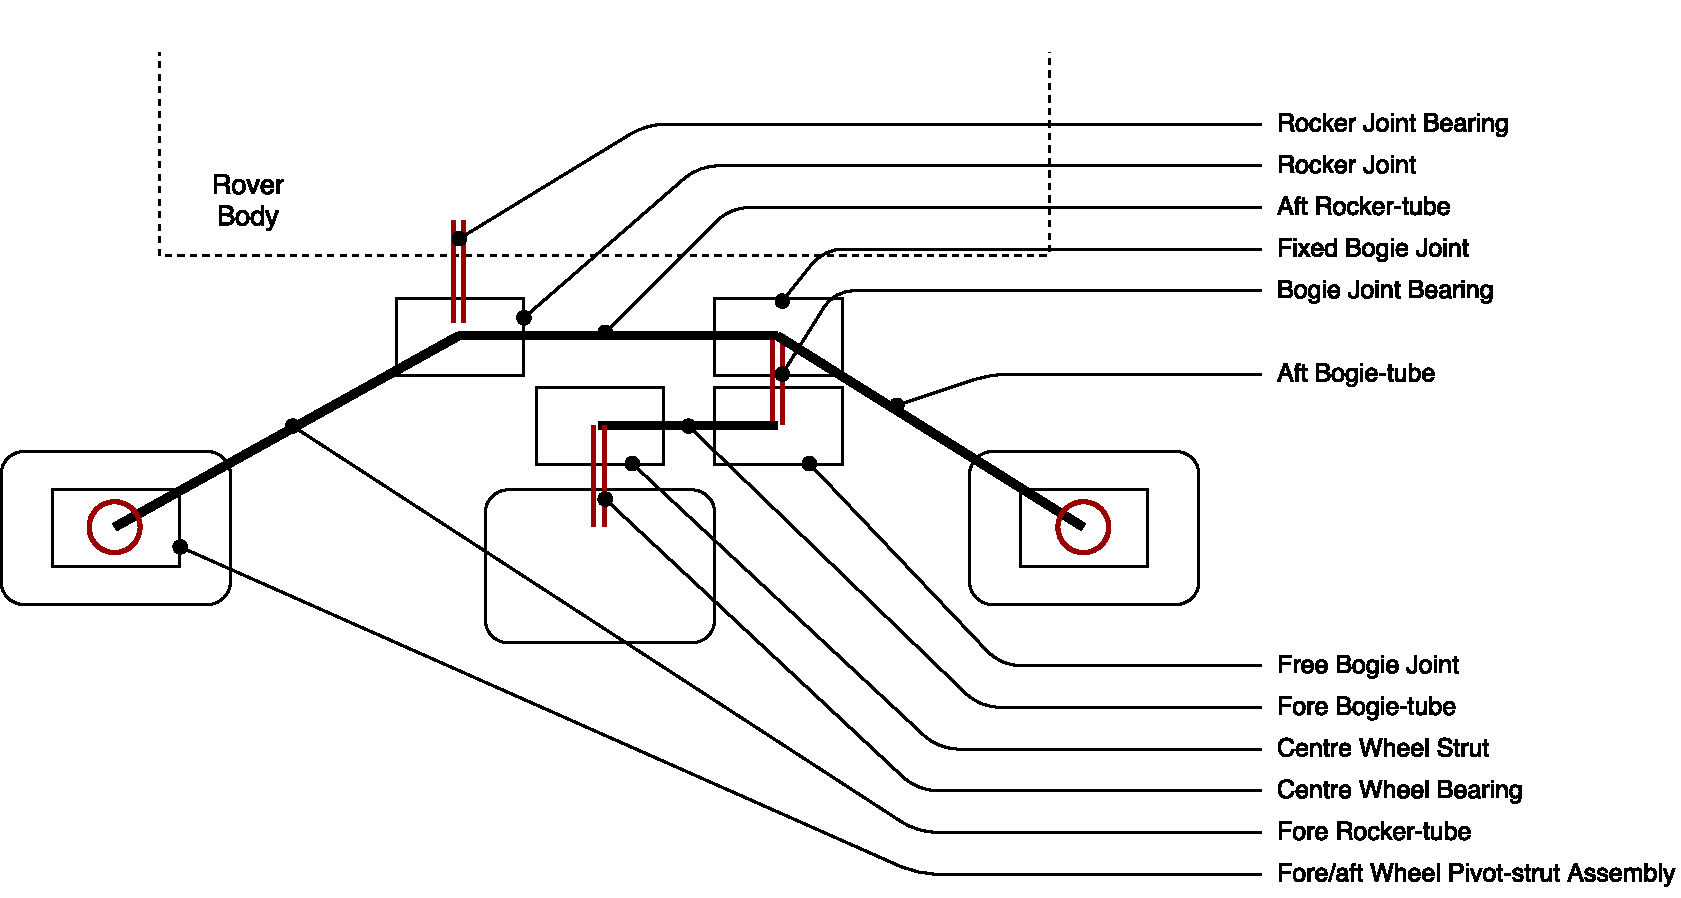
\includegraphics[width=1\linewidth]{figures/mechDesign-suspensionLinkageMap}
        \caption[Schematic diagram of a top view of the suspension system]{Schematic diagram of a top view of the suspension system}
        \label{fig:mechdesign-suspensionLinkageMap}
      \end{figure}
      
      It was noted that the ratios of the tubing or beams on \textit{Curiosity} (and rocker-bogie mechanisms in general) were important since it determined the system's range of motion, affecting the rover's ability to traverse the terrain. The reference model in \cite{nasa3Dprint} was not able to provide this kind of detail, and so the angles and positions of the centre-points of joints and axes of pivots and wheels had to be constructed from reference images of the rover. What was known was the distance of the wheels away from the side of the rover body, that the pivot centre-points were directly above the centres of the wheels and that the aft rocker-tube and the fore bogie-tube were parallel to the body of the rover in the $x$-$y$ plane. Figure \ref{fig:mechDesign-suspensionReferences} includes the images that were used to find these details.
      
      \begin{figure}[H]
      \centering
      \subfloat {
        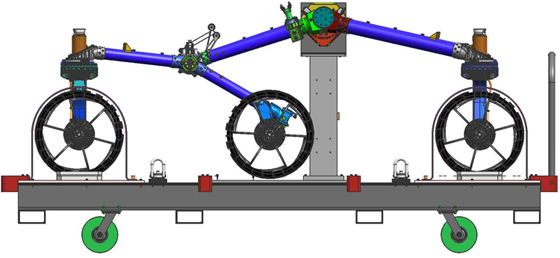
\includegraphics[width=.45\linewidth]{figures/mechDesign-suspensionReference1.jpg}
      }
      \qquad
      \subfloat {
        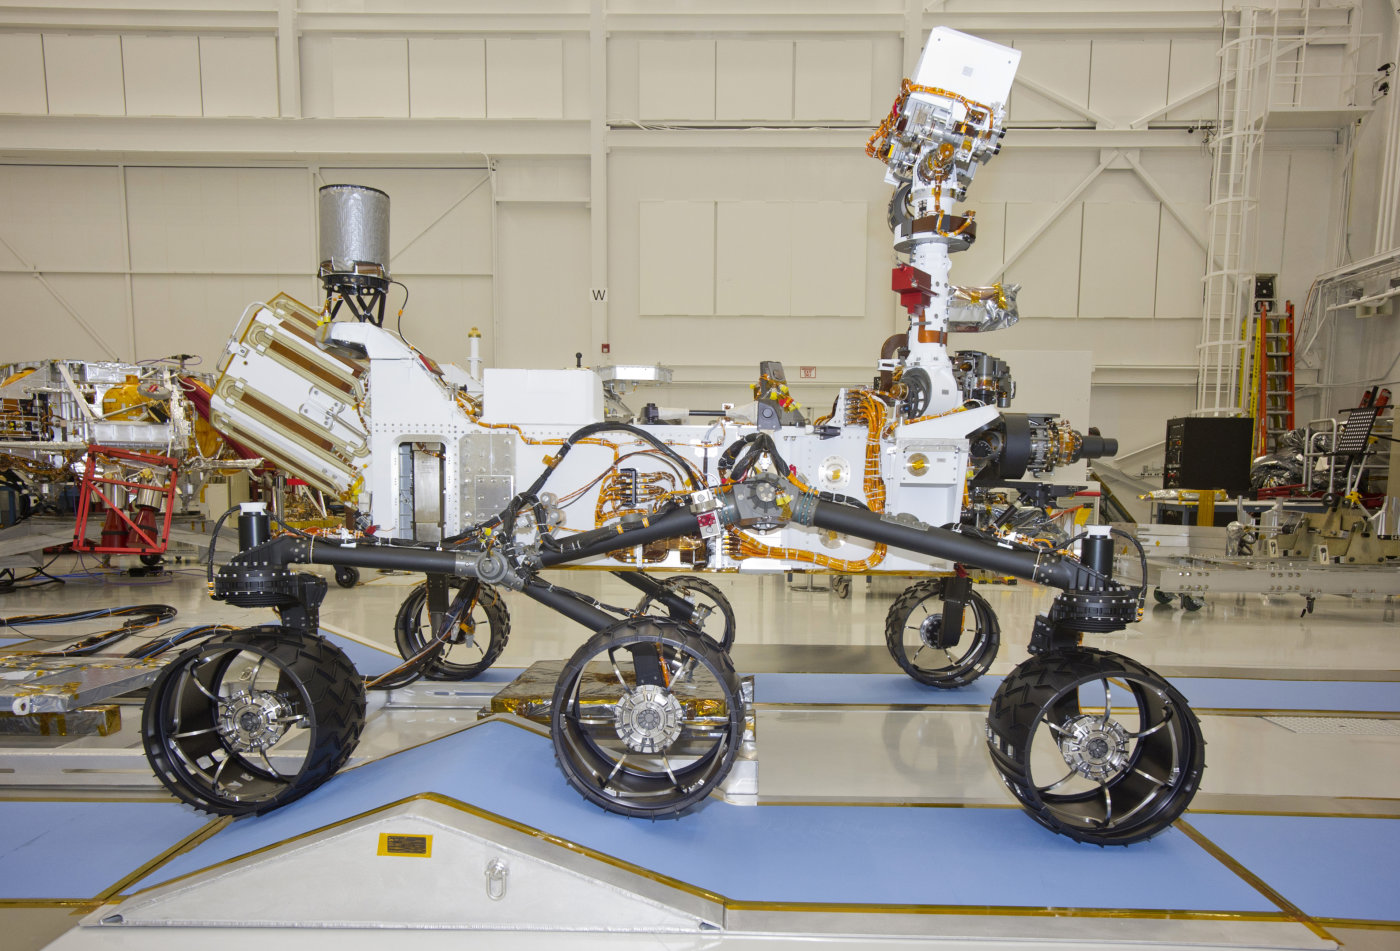
\includegraphics[width=.45\linewidth]{figures/mechDesign-suspensionReference2.jpg}
      }
      \caption[The two images used for obtaining the positions of joints and pivots of the suspension system in 3D space]{The two images used for obtaining the positions of joints and pivots of the suspension system in 3D space. \cite{fig:mechDesign-suspensionReferences1_cite} and \cite{fig:mechDesign-suspensionReferences2_cite} respectively.}
      \label{fig:mechDesign-suspensionReferences}
      \end{figure}
      
      The skeleton layout generated from the positional data obtained is shown in Figure~![] where a 2D sketch was created as a starting point from which a 3D sketch was formed. 
      
      ![Figure of the suspension skeleton]
      
      The joints, pivots and struts were then developed around the axes and centre-points in the sketch, a work-flow typical of the CAD package used.
      
      \subheading{Joints}\\\\
      \subheading{Wheels}\\\\
      \subheading{Pivots}\\\\
      \subheading{Struts}\\\\

      Having designed the parts around the skeleton sketch, where they were kept fixed to preserve the angle details linking them, another assembly was created into which the parts were re-added and mated in a manner more typical of the way that they would be assembled. The assembly allowed simulation of the movement and this functionality was used to analyse the assembly for interferences and to ensure that the structure moved the way it was required. Figure~[] shows the linkages positioned as if the subsystem was navigating over an obstacle.
      
      ![Figure of obstacle traversal of one side of the suspension]
      
    \subsubsection{Differential}
      - Bar
      - Hinges
      
    \subsubsection{Head and Neck}
      - Neck mount
      - Neck Hinge and Actuation
      - Head
    
    \subsubsection{Body}
    
    \subsubsection{Aesthetic Details}
    
  \subsection{Electrical Design}
    \subsubsection{Actuation}
    \subsubsection{Sensors}
    \subsubsection{Camera}
    \subsubsection{Power}
    \subsubsection{System Interfaces}
    
  \subsection{Integration of Mechanical and Electrical Designs}
    \subsubsection{Internal Electronics Mounting}
    \subsubsection{Cables and Wiring}